\usepackage{tikz}
\usepackage[absolute,overlay]{textpos}
\usepackage{pdfrender}

% % set titlepage in a TikZ node for modifications
\setbeamertemplate{title page}{%
\begin{tikzpicture}[remember picture,overlay]
\fill[blue]
  ([yshift=15pt]current page.west) rectangle (current page.south east);
\node[anchor=east] 
  at ([yshift=-50pt]current page.north east) (author)
  {\parbox[t]{.6\paperwidth}{\raggedleft%
    \usebeamerfont{author}\textcolor{orange}{%
    \textpdfrender{
    TextRenderingMode=FillStroke,
    FillColor=orange,
    LineWidth=.1ex,
    }{\insertauthor}}}};
\node[anchor=north east] 
  at ([yshift=-70pt]current page.north east) (institute)
  {\parbox[t]{.78\paperwidth}{\raggedleft%
    \usebeamerfont{institute}\textcolor{gray}{\insertinstitute}}};
\node[anchor=south west] 
  at ([yshift=-120pt]current page.west) (logo)
  {\parbox[t]{.20\paperwidth}{\raggedleft%
    \usebeamercolor[fg]{titlegraphic}\inserttitlegraphic}};
\node[anchor=east]
  at ([yshift=-30pt,xshift=-20pt]current page.east) (title)
  {\parbox[t]{\textwidth}{\raggedleft%
 \usebeamerfont{author}\textcolor{white}{%
    \textpdfrender{
    TextRenderingMode=FillStroke,
    FillColor=white,
    LineWidth=.25ex,
    LineJoinStyle=1,
    Flatness=20,
    RenderingIntent=Perceptual,
    }{\inserttitle}}}};
\node[anchor=east]
  at ([yshift=-60pt,xshift=-20pt]current page.east) (subtitle)
  {\parbox[t]{.5\paperwidth}{\raggedleft\usebeamerfont{subtitle}\textcolor{black}{\insertsubtitle}}};
\end{tikzpicture}
}
\titlegraphic{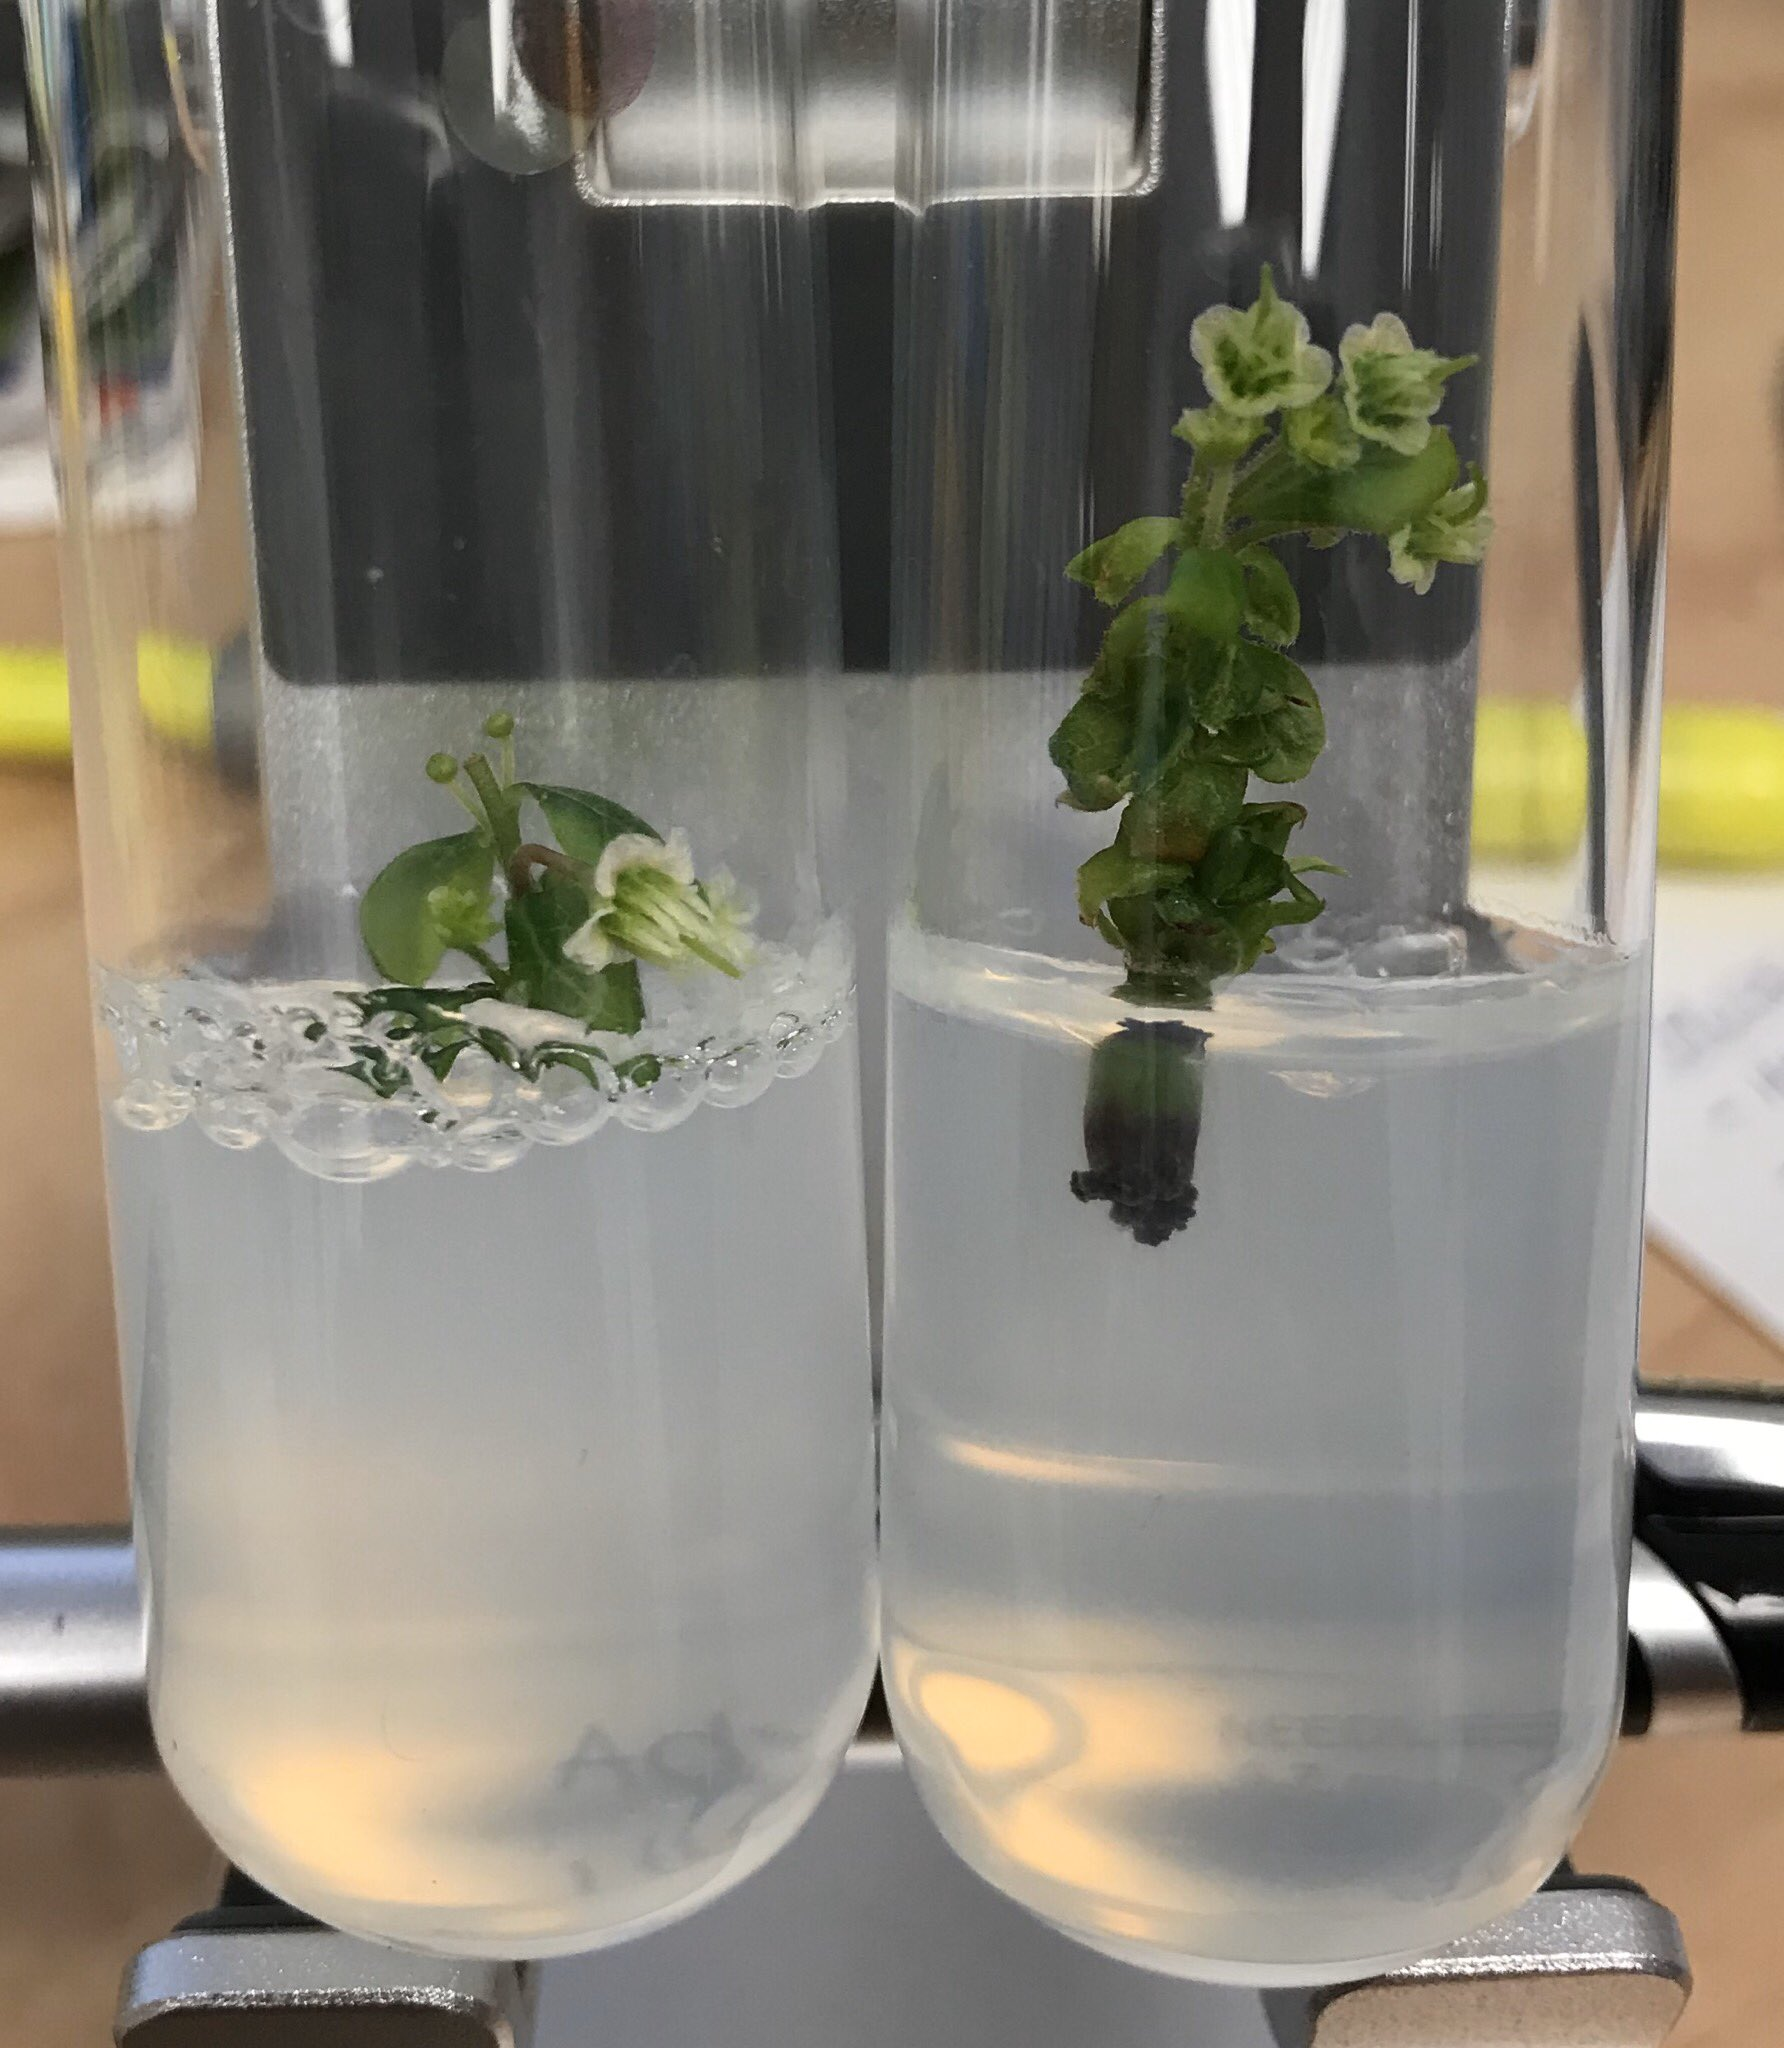
\includegraphics[width=7cm]{04-tissue_culture_techniques_vaccinium-plant.jpeg}}

% % set background image if you will
% \usebackgroundtemplate%
% {%
%     \includegraphics[width=\paperwidth,height=\paperheight]{02-dna_modification_background_dna_helix.jpg}%
% }

% % set caption font size
% % note that beamer presentation native captions have their own configs
% \usepackage{caption}
% \captionsetup{font=footnotesize}

% this font option is amenable for beamer
\setbeamerfont{caption}{size=\tiny}

% some beamer themes naturally might not support navigation symbols
% \setbeamertemplate{navigation symbols}{} % remove navigation symbols

\setbeamertemplate{footline}[page number] % insert page number in footline

% \setbeamertemplate{navigation symbols}{slide} % insert slide indication in navigation
% \setbeamertemplate{navigation symbols}{frame} % insert frame indication in navigation
% \setbeamertemplate{navigation symbols}{section} % insert section indication in navigation
% \setbeamertemplate{navigation symbols}{subsection} % insert subsection indication in navigation

% \AtBeginSubsection{} % supress subsection display
